\documentclass{beamer}

%\usetheme{Singapore}
%\usetheme{Madrid}
\usetheme{simpledso}

\usepackage{lmodern}
\usepackage[scale=2]{ccicons}

% TODO: 
%   position adjustement
%   change colours
%       

% Watermark background (simple theme)
\setwatermark{\includegraphics[height=8cm]{img/ntua.png}}

\newcommand\FourQuad[4]{
    \begin{minipage}[b][.45\textheight][t]{.50\textwidth}\centering#1\end{minipage}\hfill%
    \begin{minipage}[b][.45\textheight][t]{.50\textwidth}\centering#2\end{minipage}\\[0.9em]
    \begin{minipage}[b][.45\textheight][t]{.50\textwidth}\centering#3\end{minipage}\hfill
    \begin{minipage}[b][.45\textheight][t]{.50\textwidth}\centering#4\end{minipage}%
}

\setbeamerfont{caption}{size=\scriptsize}

\title{Routine Analysis of all available GNSS Stations in Greece:}
\subtitle{Data, products and preliminary results}
%\date{\today}
\date{}
\author{X. Papanikolaou, \emph{\underline{D. Anastasiou}}, A. Marinou, V. Zacharis and D. Paradissis}
\institute{National Technical University of Athens\\Dionysos Satellite Observatory\\\url{http://dionysos.survey.ntua.gr}}

\begin{document}

%%
%% TITLE PAGE
%%
\begin{frame}[plain]
\maketitle
\begin{block}{}
    \begin{center}
    \textbf{The Volcanic and Geodynamic Field of the South Aegean}\\
    International Workshop, Pyrgos, Santorini Isl., Greece \\
    May 20-22, 2015
    \end{center}
\end{block}
\end{frame}

%%
%% TABLE OF CONTENTS
%%
\begin{frame}
    \frametitle{Table of Contents}
    \tableofcontents
\end{frame}

\section{Introduction}

\begin{frame}\frametitle{Introduction}\framesubtitle{Past couple of years \dots}

Dionysos Satellite Observatory and Higher Geodesy Laboratory of the National Technical University of Athens, have developed an
automated processing scheme to accommodate the daily analysis of all available continuous GNSS stations in Greece.
\\
This daily analysis process, is implemented for the last two years, yielding results which help us further understand the complicated
tectonic setting of Greece and nearby regions.
\\
Important results, include:
\begin{itemize}
    \item the recent volcanic activity in \emph{Santorini} (e.g. \cite{papoutsis}),
    \item the 2014 \emph{Kefallonia} earthquakes (e.g. \cite{sarkefalonia}, \cite{sakkas})
\end{itemize}

\end{frame}

\begin{frame}\frametitle{Introduction}\framesubtitle{Currently}

    In the last months this platform has been upgraded, to include:

    \begin{itemize}
        \item more GNSS stations, divided into sub-networks,
        \item manipulation, archiving \& dissemination of GNSS data files,
        \item new processing capabilities (e.g. near real-time solutions, GPS+GLONASS processing),
        \item automatic archiving and publishing of results (via a dedicated web-site),
        \item integration with GSAC (\cite{gsac}) and MySQL databases,
        \item new results and products
    \end{itemize}

The platform was in practice re-designed \& re-implemented.

\end{frame}

\section{The Website Structure}

\begin{frame}\frametitle{The Platform}\framesubtitle{}

    Key idea : \textbf{Interconnection between the Processing Scheme, a DataBase system, GSAC interface and a dedicated WebSite.}

  \begin{columns}
    \column{.5\textwidth}
    \begin{figure}
        \begin{center}
        \includegraphics[width=.8\textwidth]{img/flowc.png}
        \caption{Flowchart of the individual platform modules.}
        \label{fig:mits}
        \end{center}
    \end{figure}
    \column{.5\textwidth}
    \begin{figure}
        \begin{center}
        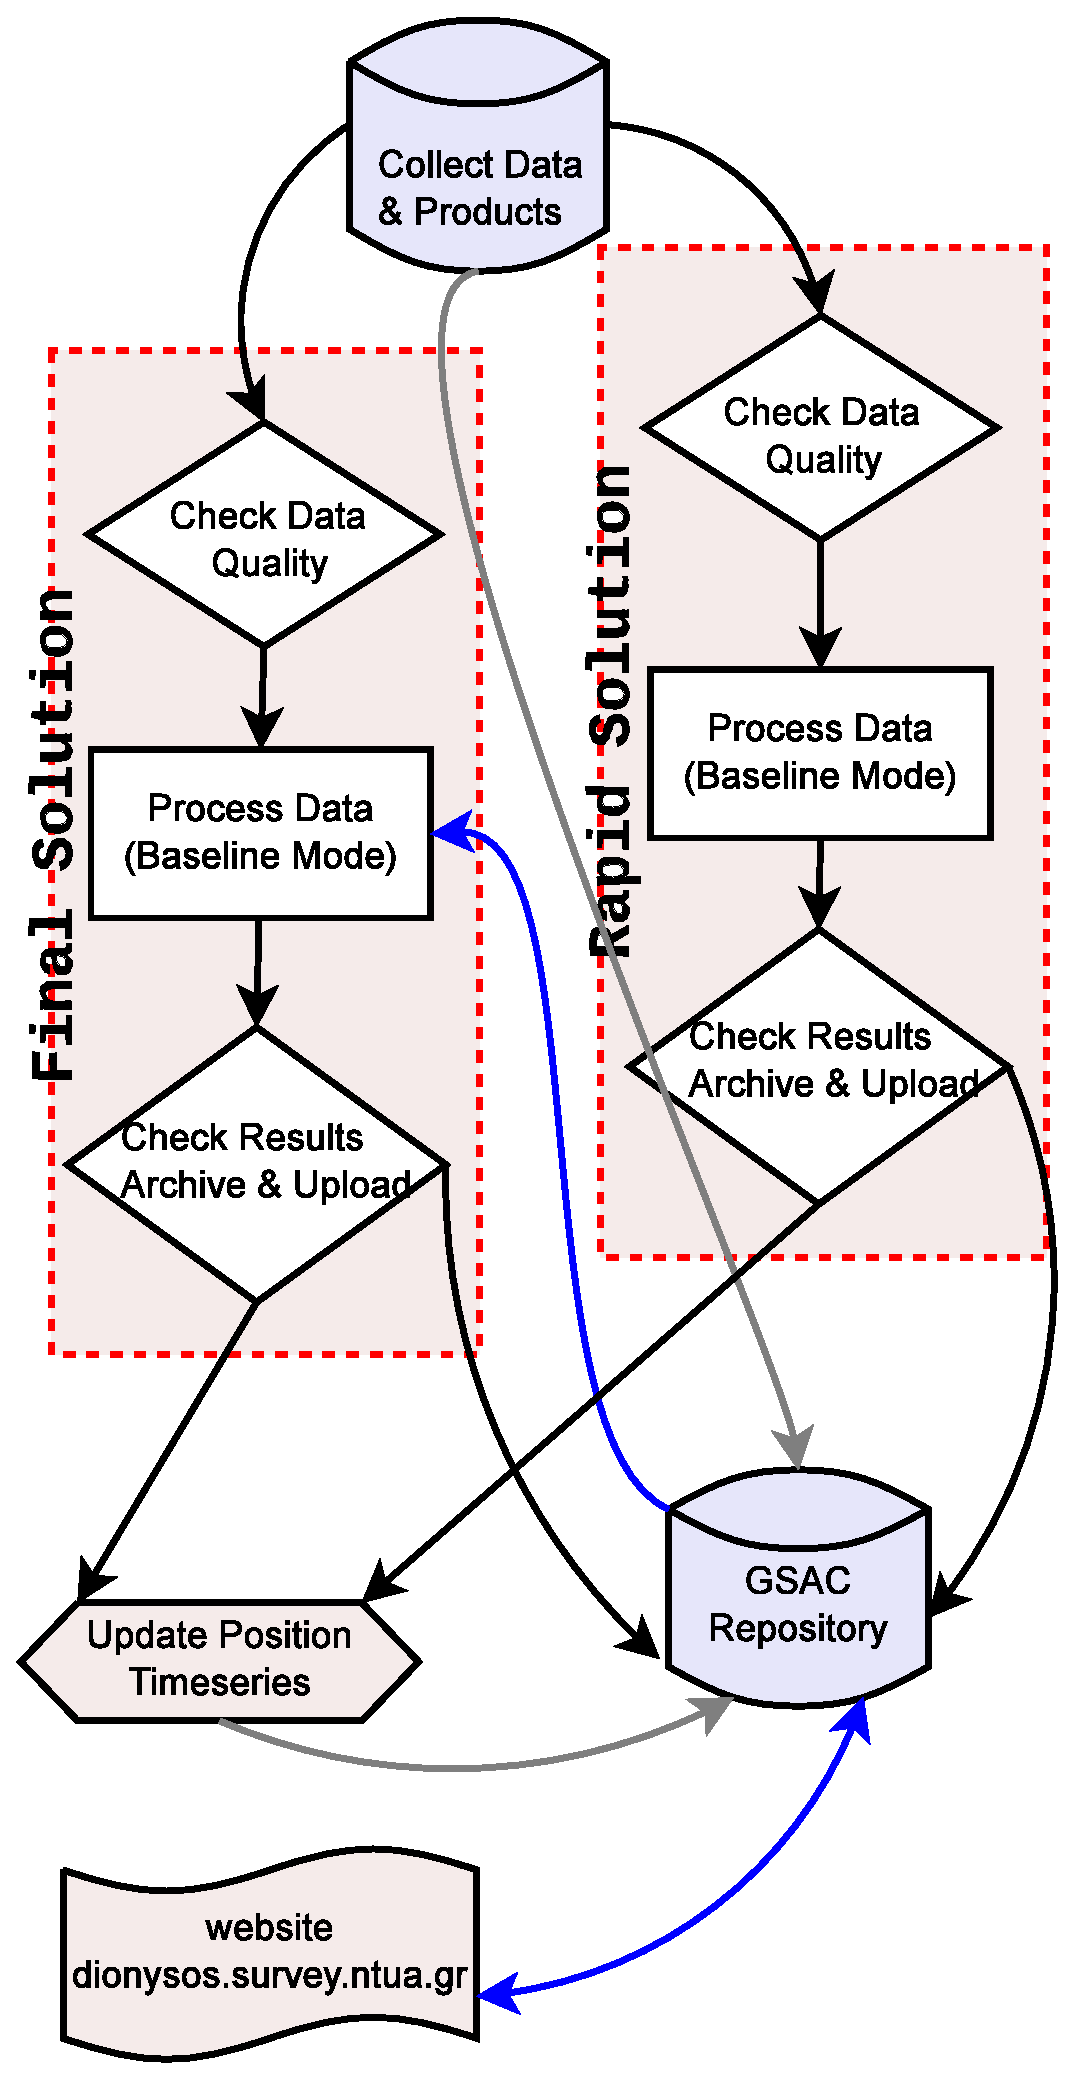
\includegraphics[width=.5\textwidth]{img/Diagram1.eps}
        \caption{Flowchart of the processing scheme.}
        \label{fig:dgrm}
        \end{center}
    \end{figure}
  \end{columns}

\end{frame}

\begin{frame}\frametitle{Sitemap}\framesubtitle{}

The sitemap, depicting the inner structure and modules of the website. It is worth noting that
it takes three individual computers (one of which virtual) to produce the final result.

    \begin{figure}
        \begin{center}
        \includegraphics[width=.7\textwidth]{img/sitemap.png}
        \caption{Website's sitemap.}
        \label{fig:mits}
        \end{center}
    \end{figure}

\end{frame}

\section{Data}

\begin{frame}\frametitle{Data}\framesubtitle{Collaborating Institutes}

Apart from NTUA, various other institutes (both Greek and from abroad) have installed and maintain
GPS/GNSS networks and provide us with data (or help us collect it)

\begin{itemize}
    \item Center for Observation and Modeling of Earthquakes, Volcanoes, and Tectonics (COMET), see \url{http://comet.nerc.ac.uk/}
    \item Corinth Rift Laboratory\footnotemark see \url{http://webobs.crlab.eu/}
    \item Institute of Geodynamics, National Observatory of Athens
    \item Tree Company (TOPCON)
    \item UNAVCO
    \item Massachusetts Institute of Technology (MIT)
\end{itemize}

\footnotetext[1]{Corinth Rift Laboratory project is a  is based on the cooperation of various european institutions that merge their efforts to study fault mechanics and related hazards in this natural laboratory. See \url{http://147.102.110.58/beta2/src/_projects/crl/}}
\end{frame}

\begin{frame}\frametitle{Data}\framesubtitle{Reception \& Manipulation}

  \begin{columns}
    \column{.7\textwidth}
    \begin{figure}
        \begin{center}
        \includegraphics[width=1.0\textwidth]{img/koko.eps}
        \caption{Flowchart of the processing scheme.}
        \label{fig:dgrm}
        \end{center}
    \end{figure}
    \column{.29\textwidth}
        \begin{itemize}
        %\item $\sim$ 150 data files processed daily (twice),
        \item 31 sites manipulated by DSO (reception, archiving \& RINEXing),
        \item dissemination via GSAC repository \& ftp site,
        \item infrastructure needs updating for some stations
    \end{itemize}
\end{columns}

\end{frame}

\begin{frame}\frametitle{Data}\framesubtitle{Dissemination}

    Users can download the data either via the \textbf{GSAC repository} of through our \textbf{ftp site}.

  \begin{columns}
    \column{.6\textwidth}
    \begin{figure}
        \begin{center}
        \includegraphics[width=1.0\textwidth]{img/gsac.png}
        \caption{Available RINEX files for 10/05/15 in GSAC repository.}
        \label{fig:mits}
        \end{center}
    \end{figure}
    \column{.4\textwidth}
    Note the availability of 1Hz data files for some of the stations. Currently 4 sites at Corinth Rift
    deliver such high-rate data.
  \end{columns}

\end{frame}

\section{Processing}

\begin{frame}\frametitle{Processing}\framesubtitle{General}

    All available data are routinely processed via Bernese \texttt{GNSS Software v5.2} (\cite{bpe}).
    
    Note that the data are divided into 4 sub-networks based primarily on their spatial distribution, 
    thus allowing a more efficient, homogenous and robust analysis scheme.
    
    Each sub-network is processed twice:
    \begin{itemize}
    \item just a few hours after the end of day using ultra-rapid products and
    \item after a time lag of 20 days using final products
    \end{itemize}

    Thus we are able to use ultra-rapid results as a-priori values for the final run.

\end{frame}

\begin{frame}\frametitle{Processing}\framesubtitle{Some Options}

    We strive to keep our processing options and models in close accordance to the IGS\footnotemark analysis centers.

    \begin{itemize}
    \item Reference frame : follow IGS realization $\Rightarrow$ currently IGb08 (\cite{igb08}) via three no-net-translation conditions imposed on a set of
    selected stations.
    \item Double-difference approach, ambiguities resolved to integers (when possible); algorithm depends on baseline length.
    \item Tropospheric mapping function : VMF1 (\cite{vmf1}).
    \item Ionospheric information is either extracted from CODE\footnotemark models, 
    or from NTUA's ultra-rapid solution.
    \item Absolute antenna calibration model (current IGS .atx).
    \item Sampling rate 30seconds, cut-off angle 7$^{\circ}$, iterative residual check.
    \end{itemize}

\footnotetext[1]{International GNSS Service}
\footnotetext[2]{Center for Orbit Determination in Europe}
\end{frame}

\begin{frame}\frametitle{Spatial Distribution}\framesubtitle{}

    \begin{figure}
        \begin{center}
        \includegraphics[width=.7\textwidth]{img/grnets.jpg}
        \caption{Stations processed by DSO.}
        \label{fig:mits}
        \end{center}
    \end{figure}

\end{frame}

\begin{frame}\frametitle{Processing}\framesubtitle{Results \& Products (1/2)}

    Analysis Results and Products include :

    \begin{itemize}
    \item SINEX\footnotemark
    \item Normal Equation Files
    \item Tropospheric SINEX,
    \item TEC maps,
    \item Coordinate estimates,
    \item Processing summary reports,
    \item Various plots and (quality) statistics ...
    \end{itemize}

    \begin{block}{Dissemination}
        %\begin{verbatim}
        Our goal is to make all products available via the GSAC repository;
        still some work to be done.
        %\end{verbatim}
    \end{block}

\footnotetext[2]{Solution (Software/technique) INdependent EXchange Format}
\end{frame}

\begin{frame}\frametitle{Processing}\framesubtitle{Results \& Products (2/2)}

    \FourQuad
    {
        \begin{figure}[t]
            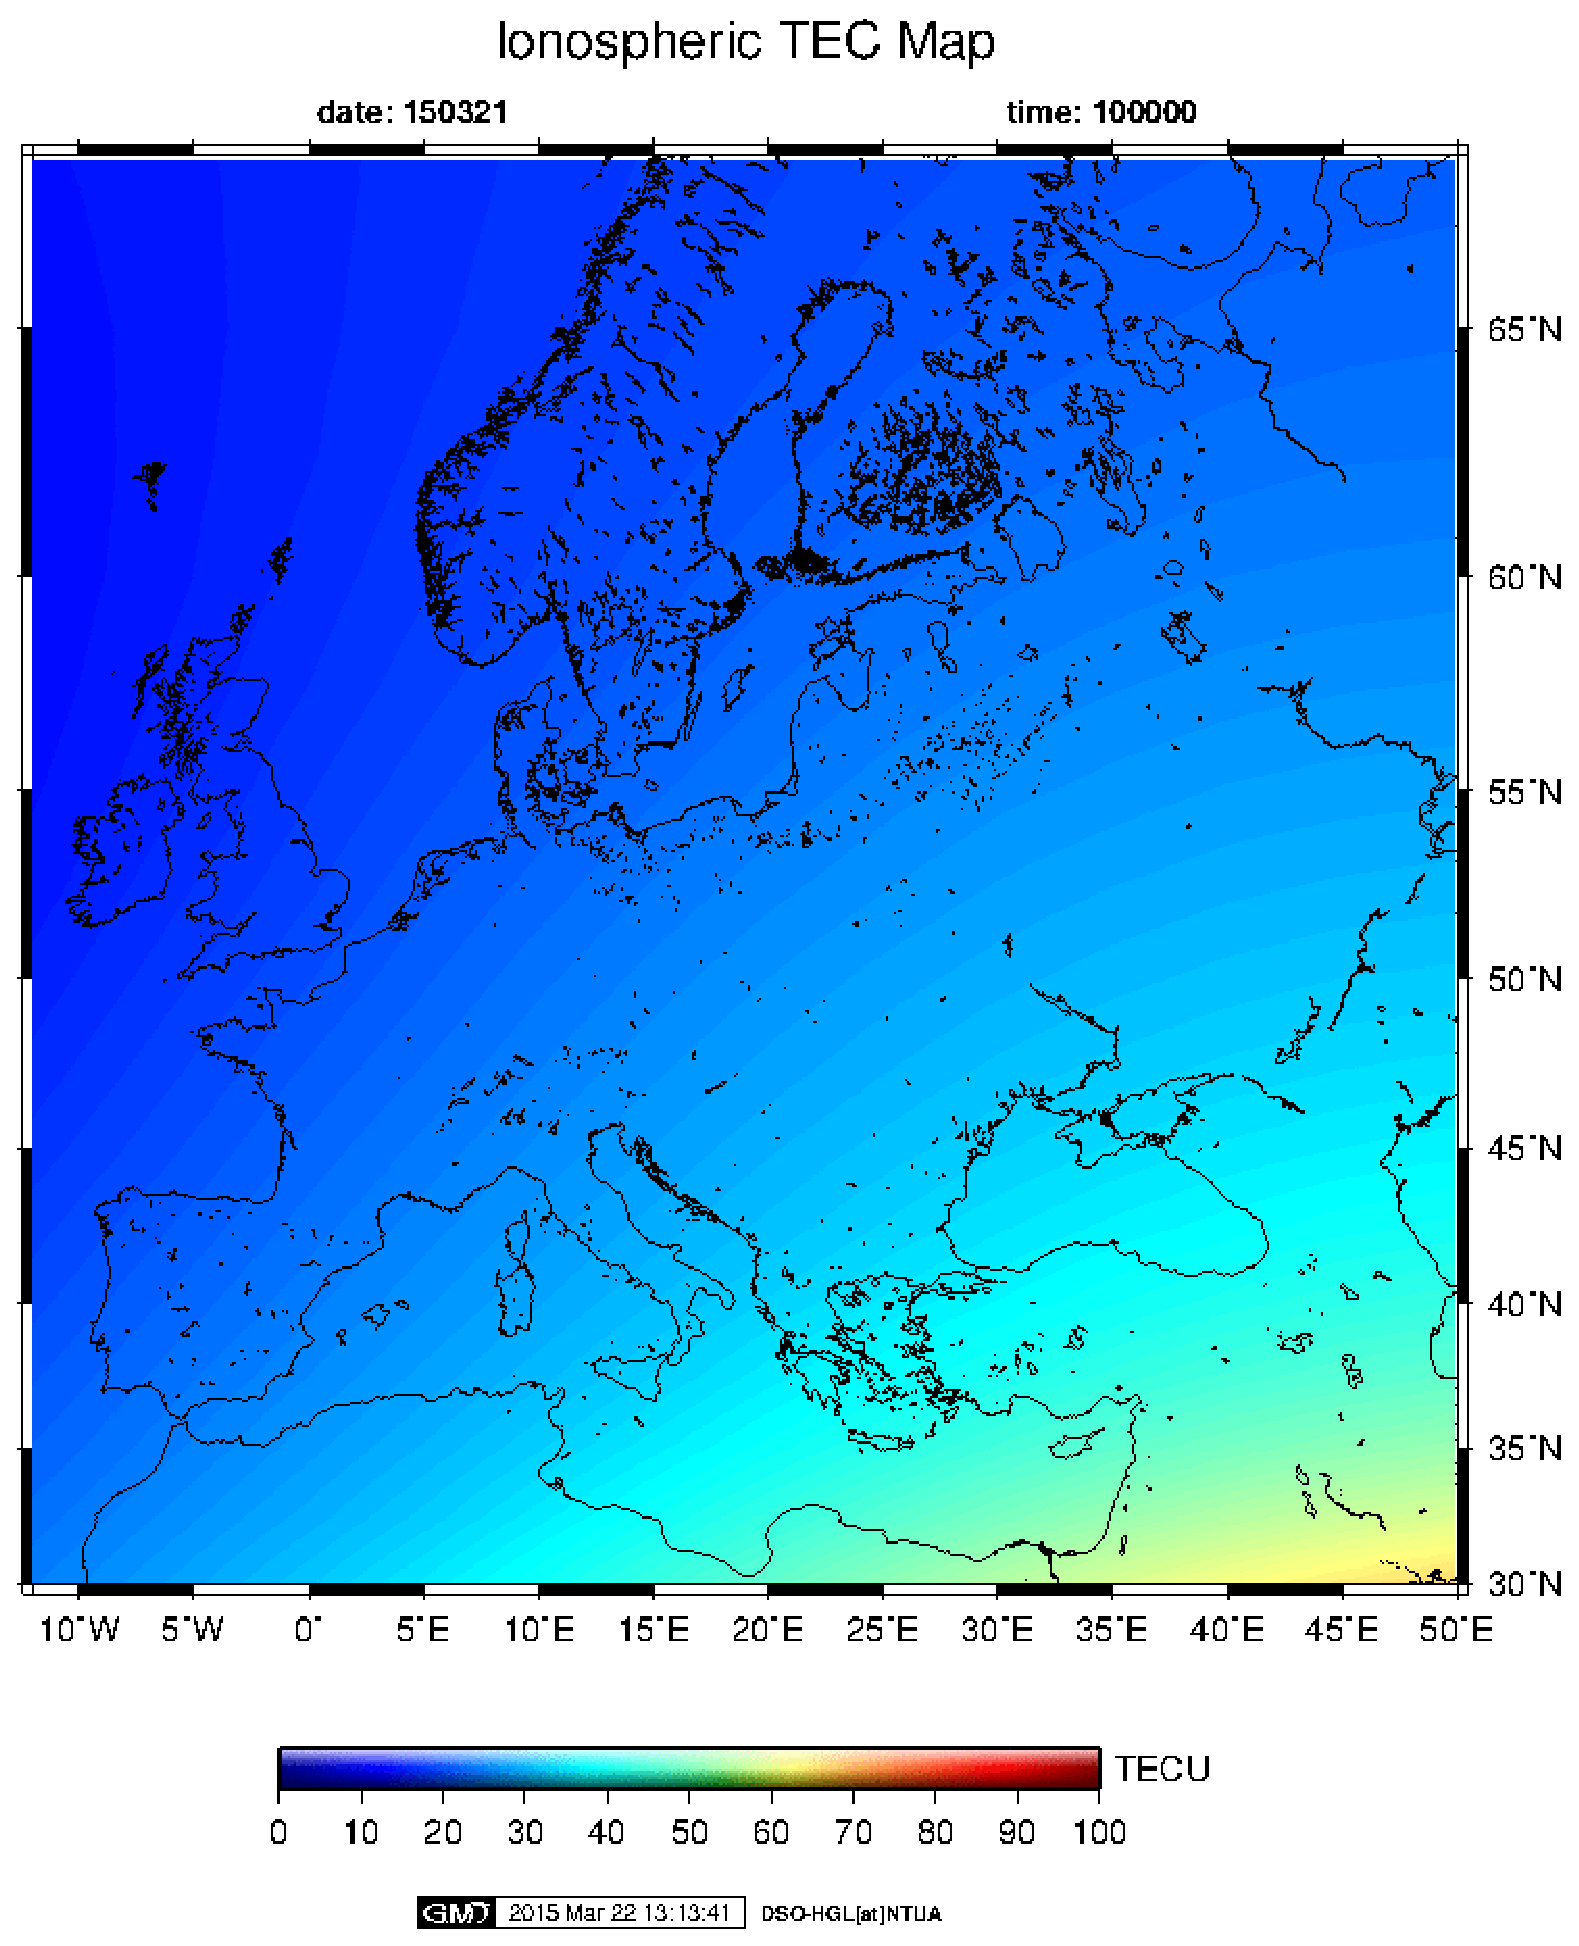
\includegraphics[width=.55\linewidth]{img/koko-5.eps}
        \end{figure}
    }
    {
        \begin{figure}[t]
            \includegraphics[width=.8\linewidth]{img/eu-greece-15065-fin-proc.eps}
        \end{figure}
    }
    {
        \begin{figure}[b]
            \includegraphics[width=.9\linewidth]{img/vlsm-mod.png}
        \end{figure}
    }
    {
        \begin{figure}[b]
            \includegraphics[width=.7\linewidth]{img/santorini_velocities_new.eps}
        \end{figure}
    }

\end{frame}

\section{TimeSeries Analysis}

\begin{frame}\frametitle{Time Series Analysis}\framesubtitle{How it's done}

    Raw time-series files, per station, are updated (twice per day) with the newest coordinate estimates.

    DSO has designed and developed a time-series analysis tool, to estimate:
    \begin{itemize}
    \item tectonic velocities,
    \item offsets (jumps),
    \item velocity changes,
    \item annual and semi-annual harmonics (amplitudes)
    \end{itemize}

    Each site has a dedicated webpage, depicting its time-series analysis information 
    (including raw and modeled ts, as well as residuals).

\end{frame}

\begin{frame}\frametitle{Time Series Analysis}\framesubtitle{Results}

    Time-Series webpage for station \texttt{lemn}; the earthquake at May-2014 is evident.

  \begin{columns}
    \column{.5\textwidth}
    \begin{figure}
        \begin{center}
        \includegraphics[width=1.0\textwidth]{img/lemn1-nbg.png}
        \caption{Time-series for station lemn.}
        \label{fig:mits}
        \end{center}
    \end{figure}
    \column{.5\textwidth}
    \begin{figure}
        \begin{center}
        \includegraphics[width=1.0\textwidth]{img/lemn2-nbg.png}
        \caption{Time-series residuals for station lemn.}
        \label{fig:mits}
        \end{center}
    \end{figure}
  \end{columns}

\end{frame}

\section{Meta-Products}

\begin{frame}\frametitle{Meta-Products}\framesubtitle{What else gets on the web}

    The website also includes several other products and/or meta-products, including
    (but not limited to):

  \begin{itemize}
    \item data files quality reports,
    \item skyplots,
    \item network analysis statistics (\#of stations, ambiguities resolved, etc $\dots$),
    \item processing reports in various formats (Docbook, xml, ascii),
    \item dedicated web-pages for phenomena of interest (e.g. Kefallonia earthquake),
    \item station log files,
    \item ionospheric remote sensing, animated TEC maps,
    \item maps
  \end{itemize}

\end{frame}

\begin{frame}\frametitle{Meta-Products}\framesubtitle{Examples}

    \FourQuad
    {
        \begin{figure}[t]
            \includegraphics[width=.75\linewidth]{img/kefa1-nbg.png}
            \caption{Webpage for the Kefallonia earthquakes.}
        \end{figure}
    }
    {
        \begin{figure}[t]
            %\includegraphics[width=.5\linewidth]{img/uranus-15087-f-greece.png}
            \includegraphics[width=.75\linewidth]{img/ambs1.png}
            \caption{Processed baselines for network URANUS.}
        \end{figure}
    }
    {
        \begin{figure}[b]
            \includegraphics[width=.45\linewidth]{img/ZIMM-20150328-cf2sky.png}
            \caption{Skyplot/Multipath for station zimm.}
        \end{figure}
    }
    {
        \begin{figure}[b]
            \includegraphics[width=.65\linewidth]{img/greece-sta.png}
            \caption{Station availability for network GREECE.}
        \end{figure}
    }

\end{frame}

\section{Integration of Results}

\begin{frame}\frametitle{Data Availability (1/2)}\framesubtitle{}

Data availability for processed sites; Note the heavy influence of URANUS network,
which only has a limited time-span.

  \begin{columns}
    \column{.5\textwidth}
    \begin{figure}
        \begin{center}
        \includegraphics[width=1.0\textwidth]{img/freqs.png}
        \caption{Data-span histogram for all processed stations ($\sim$180).}
        \label{fig:mits}
        \end{center}
    \end{figure}
    \column{.5\textwidth}
    \begin{figure}
        \begin{center}
        \includegraphics[width=1.0\textwidth]{img/greece-freqs.png}
        \caption{Data-span histogram for network GREECE ($\sim$45).}
        \label{fig:mits}
        \end{center}
    \end{figure}
  \end{columns}

\end{frame}

\begin{frame}\frametitle{Data Availability (2/2)}\framesubtitle{}

    Time-Series depicting the number of processed stations at DSO.

    \begin{figure}
        \begin{center}
        \includegraphics[width=.8\textwidth]{img/tspan.png}
        \caption{Number of processed stations.}
        \label{fig:mits}
        \end{center}
    \end{figure}

    \textbf{Note} that the reduction after the 2\textsuperscript{nd} semester of 2014, is partly
    due to our re-deployment of the processing/publishing sheme.

\end{frame}

\begin{frame}\frametitle{Velocity Field}\framesubtitle{}

    \begin{figure}
        \begin{center}
        \includegraphics[width=.7\textwidth]{img/testvel.jpg}
        \caption{Velocity Field.}
        \label{fig:mits}
        \end{center}
    \end{figure}

\end{frame}

\section{Future Work}
\begin{frame}\frametitle{Todo \dots}\framesubtitle{}

    \begin{itemize}
        \item Archive, clear \& publish old GPS data.
        \item Re-process old data with new software/models.
        \item Upgrade in-situ infrastructure (hopefully will be done within $\sim$ 3 months).
        \item Routine analysis of tide-gauge data.
        \item Integrate results with other methods (e.g. InSAR, terrestrial data, tide-gauges)\footnotemark.
        \item Model post-seismic decay (in time-series analysis).
        \item Publish all products/results via DSO's GSAC repository.
        \item Explore Real-Time capabilities.
        \item Upgrade DSO infrastructure (computing power \& storage).
    \end{itemize}

    \begin{block}{}
        \begin{center}
        More data \& collaborations !!
        \end{center}
    \end{block}

\footnotetext[2]{Already being explored in PhD dissertations (D. Anastasiou, S. Alatza, V. Zacharis).}
\end{frame}

\section{Web Resources}

\begin{frame}\frametitle{Web Resources}\framesubtitle{Visit, Browse, Interact, Comment}

\begin{itemize}
    \item \textbf{Dionysos Satellite Observatory} \url{http://dionysos.survey.ntua.gr/}  %%{http://dionysos.survey.ntua.gr/}
    \item \textbf{GSAC repository} \url{http://dionysos.survey.ntua.gr/dsoportal/_datacenter/gsacrepos.html} %%{http://dionysos.survey.ntua.gr/dsoportal/\_datacenter/gsacrepos.html}
    \item \textbf{Ftp site} \url{http://dionysos.survey.ntua.gr/dsoportal/_datacenter/ftpdata.html}  %%{http://dionysos.survey.ntua.gr/dsoportal/\_datacenter/ftpdata.html}
    \item \textbf{Kefallonia earthquake} \url{http://dionysos.survey.ntua.gr/dsoportal/_projects/supersites/cephalonia/}  %%{http://dionysos.survey.ntua.gr/dsoportal/\_projects/supersites/cephalonia/}
    \item \textbf{Ionospheric Remote Sensing} \url{http://dionysos.survey.ntua.gr/dsoportal/_projects/IonoRemSens/}  %%{}
\end{itemize}

We would be happy to hear any comments and/or suggestions.

\end{frame}

\section{Thank you}

\begin{frame}\frametitle{}\framesubtitle{}
    \begin{center}
    Thank you very much for your attention !
    \end{center}
\end{frame}

\begin{frame}[allowframebreaks]
  \frametitle<presentation>{References}
  \begin{thebibliography}{10}

%  \beamertemplatebookbibitems
%  \bibitem{Autor1990}
%    A.~Autor.
%    \newblock {\em Introduction to Giving Presentations}.
%    \newblock Klein-Verlag, 1990.

  \beamertemplatearticlebibitems

    %% Bernese
    \bibitem{bpe}
    Dach R., Hugentobler U., Fridez P., Meindl M.
    \newblock Bernese GPS Software Version 5.0
    \newblock {\em Astronomical Institute, University of Bern}, 2007.

    %% Papoutsis, Santorini
    \bibitem{papoutsis}
    Papoutsis I., Papanikolaou X., Floyd M., Ji K. H., Kontoes C., Paradissis D., Zacharis V.
    \newblock Mapping inflation at Santorini volcano, Greece, using GPS and InSAR
    \newblock {\em Geophysical Research Letters}, 40(2):267-272, 2013

    %% Sakkas, Kephalonia
    \bibitem{sakkas}
    Sakkas V., Lagios E.
    \newblock Fault modelling of the early-2014 $\sim$ M6 Earthquakes in Cephalonia Island (W. Greece) based on GPS measurements
    \newblock {\em Tectonophysics}, Volumes 644–645,184-196, 2015, Pages 184-196

    %% Diaforoi, sar kephalonia
    \bibitem{sarkefalonia}
    Merryman Boncori J.P., Papoutsis I., Pezzo G., Tolomei C., Atzori S., Ganas A., Karastathis V., Salvi S., Kontoes C., Antonioli A.
    \newblock The February 2014 Cephalonia Earthquake (Greece): 3D Deformation Field and Source Modeling from Multiple SAR Techniques
    \newblock {\em Seismological Research Letters}, Vol.86(1), 2015

    %% Unavco GSAC
    \bibitem{gsac}
    UNAVCO
    \newblock GSAC -- Geodetic Seamless Archive Centers: Open-source Software for Geodesy Data Repositories
    \newblock {\em available at} \url{https://www.unavco.org/software/data-management/gsac/gsac.html}

    %% Unavco IGB08
    \bibitem{igb08}
    P. Rebischung
    \newblock IGb08: an update on IGS08
    \newblock {\em IGSMAIL [6663]} \url{http://igscb.jpl.nasa.gov/pipermail/igsmail/2012/007853.html}, 2012

    %% Unavco vmf1
    \bibitem{vmf1}
    Boehm J., B. Werl, and H. Schuh (2006)
    \newblock Troposphere mapping functions for GPS and very long baseline interferometry from European Centre for
    Medium-Range Weather Forecasts operational analysis data
    \newblock {\em Journal of Geophysical Research}, vol. 111, B02406, 2006

  \end{thebibliography}
\end{frame}

%\setwatermark{\fontsize{125pt}{125pt}\selectfont{Simple}}

%\begin{frame}[fragile]{watermark}
%  \framesubtitle{not only for images}

%  \begin{itemize}
%    \item You can place \emph{any} \LaTeX{} \alert{contents} as a watermark
%  \end{itemize}

%  \begin{block}{In preamble}
%    \begin{verbatim}
%     \setwatermark{\includegraphics[height=8cm]{%
%                   img/Heckert_GNU_white.png}}
%    \end{verbatim}
%  \end{block}

%  \begin{block}{Just before this frame}
%    \begin{verbatim}
%     \setwatermark{\fontsize{125pt}{125pt}%
%                   \selectfont{Simple}}
%    \end{verbatim}
%  \end{block}


%\end{frame}



%\setwatermark[hoffset=-3cm,voffset=-2cm]{\fontsize{1pt}{1pt}\selectfont{Simple}}


%\begin{frame}{Options}
%  \framesubtitle{Fine adjustement of the watermark position}

  
%  \begin{itemize}
%    \item \texttt{hoffset}
%    \item \texttt{voffset}
%  \end{itemize}
  
%  They admit any \emph{positive} or \emph{negative} spacing \alert{unit}
  
%  Note that some \alert{warnings} about \emph{badboxes} might be generated at compilation

%\end{frame}




%\begin{frame}{License}

%  \begin{block}{Get the source of this theme and the demo presentation from}

%  \begin{center}\url{http://github.com/famuvie/beamerthemesimple}\end{center}

%  \end{block}
  
%  The theme \emph{itself} is licensed under a
%  \href{http://creativecommons.org/licenses/by-sa/4.0/}{Creative Commons
%  Attribution-ShareAlike 4.0 International License}.

%  \begin{center}\ccbysa\end{center}

%\end{frame}

\end{document}